\documentclass{article}
\usepackage{geometry}
\geometry{letterpaper, margin=1in}
\usepackage[utf8]{inputenc}
\usepackage{graphicx}
\usepackage{upgreek}
\usepackage{url}
\usepackage[T1]{fontenc}
\usepackage{amsmath}
\usepackage[colorinlistoftodos]{todonotes}
\usepackage[
backend=biber,
style=ieee,
sorting=none
]{biblatex}
 
\addbibresource{assign.bib}

\title{ECE532S Digital Systems Design \\ \vspace{0.4cm}
       \Large Assignment 1 - Custom IP and Simulation \\ \vspace{0.4cm}
       \small Due: Feb 00, 2019}
\author{ }
\date{ }


\begin{document}
\maketitle
\vspace{-1cm}

Testbenches are used to simulate digital designs without the need for lengthy synthesis and implementation runs and without the need for physical hardware. Such simulation also allows you to inspect individual internal signals of the digital design and control the values of inputs over time within the testbench environment. This fine-grained signal control and observability makes simulation through testbenches the primary means to debug digital designs.

Alternative debug procedures usually involve the full synthesis and implementation procedure, the explicit connection or selection of signals to probe, and limited probing capabilities. For example, the Xilinx Vivado set of tools provides a number of debug cores which can facilitate this on-device debugging. These modes of test are more complicated, and simulation via testbenches is highly recommended.

A testbench is a module, generally written in a Hardware Descriptor Language (e.g. Verilog), that instantiates your digital design, drives it's input signals, and observes the output signals. The instantiation of your module within the testbench is often termed the \textit{Design Under Test}, or \textit{DUT}. The testbench code is generally not synthesizable into a circuit as it uses HDL constructs that have no real digital implementation.

In this assignment, you will learn to make a proper testbench for a simple digital design, create a new IP with specified behaviour, and then make another testbench to test the implemented IP.

\section{Simple Mask Module and Testbench}
\label{sec:mask}
Masks are used in hardware to clear or set specific bits in a multi-bit signal, while allowing other bits of the signal to pass unaffected. When masking bits to zero, the convention is that any bits within the mask which are set to 0 should force the signal to zero, and any bits which are set to 1 should allow the signal to pass unaffected. This is often performed using a bitwise \textit{AND} of the mask and the input signal. In this part of the assignment, you will implement such a masking module.

\subsection{Problem}
\label{sec:mask_prob}
You must construct a simple masking module, conforming to the following Verilog interface:

\begin{verbatim}
module mask532
(
  input [4:0]   n,        // number of bits to mask
  input [31:0]  value_in, // input value
  output [31:0] value_out // output value
);
\end{verbatim}

This module has a 32-bit input value and a 32-bit output value. The output value should be a masked version of the input value. The 5-bit input value \textit{n} specifies the number of bits to mask from the input value. Specifically, the \textit{n} most-significant bits of the input should be masked to zero on the output signal. For example, if the input is 0x01234567 and n is 12 (decimal), then the output should be 0x00034567.

Once you have made the module, you will need to create a testbench to test the functionality of the module (details described in next section). Look at the Vivado Simulation Tutorial~\cite{xilinxsimtut} for reference.

\subsection{Tasks}
Implement the masking module with functionality as described in Section~\ref{sec:mask_prob}. Once the module is complete, write a testbench which instantiates your mask module and tests the module for a number of input values; choose the input values such that you are reasonably confident that your module functions correctly. The testbench must simulate your module in three different ways: using the waveform viewer; using the Verilog \textit{\$display} command; and using the Verilog \textit{\$monitor} command.
\\

\begin{minipage}{\textwidth}
\noindent\textbf{Submission}\\
In your report include:
\begin{enumerate}
\item A description of why you chose the specific test inputs you used in your Verilog testbench
\item A summary of the output of each of the simulation methodologies (can be displayed as a figure)
\item A discussion comparing the different simulation methods. What are the advantages and disadvantages of each? Are there specific situations in which one would be preferable to the others?
\end{enumerate}
Submit the Verilog code for your masking module and the Verilog code for your testbench as separate files. Also, submit the the wdb file which contains the waveform from your simulation. Please include comments indicating where and how the \$display and \$monitor commands are used.
\end{minipage}


\section{Creating an AXI IP}
\label{sec:mask_ip}
In the previous section, you designed a simple digital module implementing the masking functionality. It is common in hardware design to wrap our simple module designs as IP blocks to be used in system design using the IP Integrator mode within Vivado. In this section, we will be wrapping our simple masking module using AXI interfaces to allow it to interact with other AXI interfaces on Xilinx provided IP cores. You should review the AXI standard~\cite{ambaaxispec} and the Xilinx AXI Reference Guide~\cite{xilinxaxiref} for more detailed information on the AXI standard.

\subsection{Problem}
Create a Verilog module that has the following AXI-Lite interfaces:

\begin{verbatim}
module mask_axi532
(
  input         aclk,    // clock
  input         aresetn, // asynchronous reset
  
  //AXI Slave Port
  input [31:0]  S_AXI_AWADDR,  // AXI-Lite slave write address
  input         S_AXI_AWVALID, // AXI-Lite slave write valid
  output        S_AXI_AWREADY, // AXI-Lite slave write ready
  ...                          // Rest of AXI-Lite slave signals (read and write channels)
  
  //AXI Master Port
  output [31:0] M_AXI_AWADDR,  // AXI-Lite master write address
  output        M_AXI_AWVALID, // AXI-Lite master write valid
  input         M_AXI_AWREADY, // AXI-Lite master write ready
  ...                          // Rest of AXI-Lite master signals (only write channels needed)
);
\end{verbatim}

The module has AXI clock and reset signals, and then two specific AXI-Lite interfaces (Note, not AXI4, very important distinction). The AXI-Lite slave interface accepts both read and write request and therefore should have all of the AXI-Lite channels (AW,W,B,AR,R). The AXI-Lite master interface sends only write requests, and therefore only needs to have the write channels implemented (AW,W,B).

The purpose of this module is depicted in Figure~\ref{fig:mask_ip}. The AXI-Lite slave interface connects internally to a module which contains an AXI-Lite slave interface and 4 register outputs. The four registers are the \textit{n\_value}, \textit{data\_value}, \textit{output\_addr}, and \textit{init\_write} registers, mapped to address offsets of 0, 4, 8, and 12 respectively. This AXI-slave sub-component can be implemented using the methods we've used in previous tutorials to make AXI-Lite registers. The first three of these registers should support both read and write operations, and the final register should support write operations only. In addition, the final register need only be 1-bit wide and should be set high when written to for just a single cycle before returning to a low value (this will require modification to the Xilinx provided AXI-Lite Register Verilog code).

\begin{figure}[t]
\centering
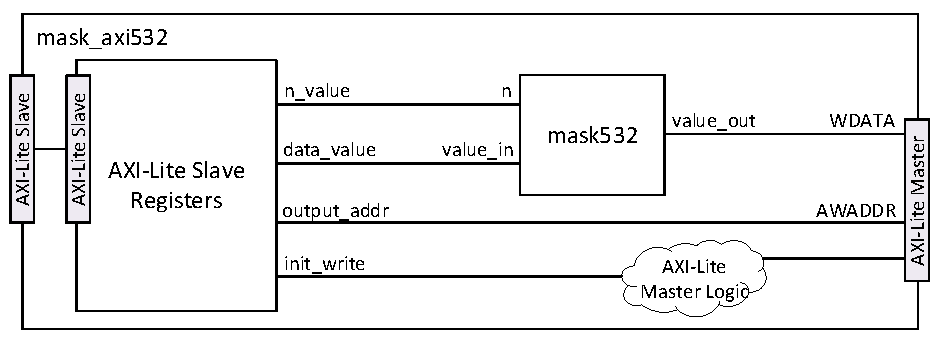
\includegraphics[width=0.8\textwidth]{mask_axi.pdf}
\caption{Specific implementation for AXI-Lite wrapped mask module}
\label{fig:mask_ip}
\end{figure}

The \textit{n\_value} and the \textit{data\_value} should be connected to the \textit{mask532} module created in Section~\ref{sec:mask}. Specifically, the signals should be connected to the \textit{n} and \textit{value\_in} ports respectively. Note, this means that the \textit{n\_value} register need only be 5-bits wide. The \textit{value\_out} signal of the \textit{mask532} module should be connected directly to the \textit{M\_AXI\_WDATA} field of the AXI-Lite master interface, thereby insuring that a masked version of the \textit{data\_value} register is written on the AXI-Lite master interface. In addition, ensure that the \textit{output\_addr} register is connected directly to the \textit{M\_AXI\_AWADDR} field of the AXI-Lite master interface.

Finally, you must implement logic that upon seeing a high value on the single-bit \textit{init\_write} register, initiates a write on the AXI-Lite master interface. This requires handshaking on the \textit{AW} signals to initiate a write, handshaking on the \textit{W} signals to send the write data, and receiving the \textit{B} write response signals correctly. Note, the \textit{init\_write} signal should stay high for a single cycle only, and thus should initiate just one write; you can ignore any \textit{init\_write} signals while a transaction is waiting to be initiated on the \textit{AW} channel.

\subsection{Tasks}
Implement the mask module which makes use of AXI-lite interfaces and the masking module you designed in Section~\ref{sec:mask}. Ensure the functionality is conformant with the above description. Once the module is complete, use the Vivado IP Packager to package your newly created IP. See the Vivado Custom IP Packaging Tutorial~\cite{xilinxpacktut} for reference.
\\

\begin{minipage}{\textwidth}
\noindent\textbf{Submission}\\
In your report include:
\begin{enumerate}
\item A short description of how you implemented the required change in the AXI-Lite slave register code which ensured that the \textit{init\_write} signal stayed set for only a single cycle when written
\item A short description of how you implemented the AXI-Lite master writing functionality
\end{enumerate}
Submit all of the Verilog files used in implementing your AXI-based masking module. Also make sure to submit the component.xml file created by the Vivado IP Packager tool. Please include sufficient comments within the Verilog such that the implement hardware is easy to understand.
\end{minipage}


\section{Simulating an AXI module IP}
Since many of the hardware modules we implement in SoC systems use AXI interfaces (i.e. in order to mate to other Xilinx IPs or microblaze processors), we need to be able to simulate hardware blocks using AXI interfaces. While we could generate testbenches which directly set the inputs of all the different AXI signals, this would be an onerous and repetitive process for every transaction. For this reason, we generally use specific verification IPs which hide the protocol complications in our testbenches. In this section, we'll use the Xilinx AXI Verification IP to test our newly created IP core. For more information, review the Xilinx AXI Verification IP product guide~\cite{xilinxvip}.

\subsection{Tasks}
Create a new Vivado project with a block diagram. Within the block diagram, instantiate a copy of your new IP, a BRAM and a BRAM controller, a Processor System Reset IP, and an AXI VIP. Configure the system such that the AXI-Lite master port of the mask IP can write to the BRAM, and the AXI VIP can read and write to the BRAM and the AXI-Lite slave port of the mask IP. All resets within the system should be connected to the Processor System Reset (which simply synchronizes reset events with the clock) and the only signals which should be external are the input to the Processor System Reset and the clock. Name your ports \textit{clk} and \textit{resetn} (i.e. the reset is active low). Note, a tcl script is provided which automates the above steps, but make sure to look through the tcl script to understand how the system is built (it will help you to simulate AXI cores in the future). Note, the tcl script will not add the mask IP you created in Section~\ref{sec:mask_ip}, so you will have to add it yourself and connect it to the two AXI interconnects.

Once the block diagram is created, generate the HDL wrapper and move on to working on the testbench. The testbench should test the functionality of the mask IP by writing to its registers and triggering it to write to the BRAM. The testbench should then check the BRAM to ensure the written values are as expected. Make sure to write a testbench that checks enough cases such that you are satisfied that the core functions as expected. For information on how to use the AXI VIP, refer to the Xilinx documentation~\cite{xilinxvip}, and to the AXI VIP tutorials available on the course page.
\\

\begin{minipage}{\textwidth}
\noindent\textbf{Submission}\\
In your report include:
\begin{enumerate}
\item A short description of your testbench functionality
\item A description of why you chose the specific test inputs you used in your Verilog testbench
\item A summary of the output of the simulation (can be displayed as a figure)
\end{enumerate}
Submit the Verilog code for your testbench as a separate file.
\end{minipage}



\newpage
\printbibliography

\end{document}
